% Options for packages loaded elsewhere
\PassOptionsToPackage{unicode}{hyperref}
\PassOptionsToPackage{hyphens}{url}
%
\documentclass[
]{article}
\usepackage{lmodern}
\usepackage{amssymb,amsmath}
\usepackage{ifxetex,ifluatex}
\ifnum 0\ifxetex 1\fi\ifluatex 1\fi=0 % if pdftex
  \usepackage[T1]{fontenc}
  \usepackage[utf8]{inputenc}
  \usepackage{textcomp} % provide euro and other symbols
\else % if luatex or xetex
  \usepackage{unicode-math}
  \defaultfontfeatures{Scale=MatchLowercase}
  \defaultfontfeatures[\rmfamily]{Ligatures=TeX,Scale=1}
\fi
% Use upquote if available, for straight quotes in verbatim environments
\IfFileExists{upquote.sty}{\usepackage{upquote}}{}
\IfFileExists{microtype.sty}{% use microtype if available
  \usepackage[]{microtype}
  \UseMicrotypeSet[protrusion]{basicmath} % disable protrusion for tt fonts
}{}
\makeatletter
\@ifundefined{KOMAClassName}{% if non-KOMA class
  \IfFileExists{parskip.sty}{%
    \usepackage{parskip}
  }{% else
    \setlength{\parindent}{0pt}
    \setlength{\parskip}{6pt plus 2pt minus 1pt}}
}{% if KOMA class
  \KOMAoptions{parskip=half}}
\makeatother
\usepackage{xcolor}
\IfFileExists{xurl.sty}{\usepackage{xurl}}{} % add URL line breaks if available
\IfFileExists{bookmark.sty}{\usepackage{bookmark}}{\usepackage{hyperref}}
\hypersetup{
  pdftitle={2.0 Multivariate Visualization Assignment},
  pdfauthor={JD Santos},
  hidelinks,
  pdfcreator={LaTeX via pandoc}}
\urlstyle{same} % disable monospaced font for URLs
\usepackage[margin=1in]{geometry}
\usepackage{color}
\usepackage{fancyvrb}
\newcommand{\VerbBar}{|}
\newcommand{\VERB}{\Verb[commandchars=\\\{\}]}
\DefineVerbatimEnvironment{Highlighting}{Verbatim}{commandchars=\\\{\}}
% Add ',fontsize=\small' for more characters per line
\usepackage{framed}
\definecolor{shadecolor}{RGB}{248,248,248}
\newenvironment{Shaded}{\begin{snugshade}}{\end{snugshade}}
\newcommand{\AlertTok}[1]{\textcolor[rgb]{0.94,0.16,0.16}{#1}}
\newcommand{\AnnotationTok}[1]{\textcolor[rgb]{0.56,0.35,0.01}{\textbf{\textit{#1}}}}
\newcommand{\AttributeTok}[1]{\textcolor[rgb]{0.77,0.63,0.00}{#1}}
\newcommand{\BaseNTok}[1]{\textcolor[rgb]{0.00,0.00,0.81}{#1}}
\newcommand{\BuiltInTok}[1]{#1}
\newcommand{\CharTok}[1]{\textcolor[rgb]{0.31,0.60,0.02}{#1}}
\newcommand{\CommentTok}[1]{\textcolor[rgb]{0.56,0.35,0.01}{\textit{#1}}}
\newcommand{\CommentVarTok}[1]{\textcolor[rgb]{0.56,0.35,0.01}{\textbf{\textit{#1}}}}
\newcommand{\ConstantTok}[1]{\textcolor[rgb]{0.00,0.00,0.00}{#1}}
\newcommand{\ControlFlowTok}[1]{\textcolor[rgb]{0.13,0.29,0.53}{\textbf{#1}}}
\newcommand{\DataTypeTok}[1]{\textcolor[rgb]{0.13,0.29,0.53}{#1}}
\newcommand{\DecValTok}[1]{\textcolor[rgb]{0.00,0.00,0.81}{#1}}
\newcommand{\DocumentationTok}[1]{\textcolor[rgb]{0.56,0.35,0.01}{\textbf{\textit{#1}}}}
\newcommand{\ErrorTok}[1]{\textcolor[rgb]{0.64,0.00,0.00}{\textbf{#1}}}
\newcommand{\ExtensionTok}[1]{#1}
\newcommand{\FloatTok}[1]{\textcolor[rgb]{0.00,0.00,0.81}{#1}}
\newcommand{\FunctionTok}[1]{\textcolor[rgb]{0.00,0.00,0.00}{#1}}
\newcommand{\ImportTok}[1]{#1}
\newcommand{\InformationTok}[1]{\textcolor[rgb]{0.56,0.35,0.01}{\textbf{\textit{#1}}}}
\newcommand{\KeywordTok}[1]{\textcolor[rgb]{0.13,0.29,0.53}{\textbf{#1}}}
\newcommand{\NormalTok}[1]{#1}
\newcommand{\OperatorTok}[1]{\textcolor[rgb]{0.81,0.36,0.00}{\textbf{#1}}}
\newcommand{\OtherTok}[1]{\textcolor[rgb]{0.56,0.35,0.01}{#1}}
\newcommand{\PreprocessorTok}[1]{\textcolor[rgb]{0.56,0.35,0.01}{\textit{#1}}}
\newcommand{\RegionMarkerTok}[1]{#1}
\newcommand{\SpecialCharTok}[1]{\textcolor[rgb]{0.00,0.00,0.00}{#1}}
\newcommand{\SpecialStringTok}[1]{\textcolor[rgb]{0.31,0.60,0.02}{#1}}
\newcommand{\StringTok}[1]{\textcolor[rgb]{0.31,0.60,0.02}{#1}}
\newcommand{\VariableTok}[1]{\textcolor[rgb]{0.00,0.00,0.00}{#1}}
\newcommand{\VerbatimStringTok}[1]{\textcolor[rgb]{0.31,0.60,0.02}{#1}}
\newcommand{\WarningTok}[1]{\textcolor[rgb]{0.56,0.35,0.01}{\textbf{\textit{#1}}}}
\usepackage{graphicx,grffile}
\makeatletter
\def\maxwidth{\ifdim\Gin@nat@width>\linewidth\linewidth\else\Gin@nat@width\fi}
\def\maxheight{\ifdim\Gin@nat@height>\textheight\textheight\else\Gin@nat@height\fi}
\makeatother
% Scale images if necessary, so that they will not overflow the page
% margins by default, and it is still possible to overwrite the defaults
% using explicit options in \includegraphics[width, height, ...]{}
\setkeys{Gin}{width=\maxwidth,height=\maxheight,keepaspectratio}
% Set default figure placement to htbp
\makeatletter
\def\fps@figure{htbp}
\makeatother
\setlength{\emergencystretch}{3em} % prevent overfull lines
\providecommand{\tightlist}{%
  \setlength{\itemsep}{0pt}\setlength{\parskip}{0pt}}
\setcounter{secnumdepth}{-\maxdimen} % remove section numbering
\usepackage{float}
\let\origfigure\figure
\let\endorigfigure\endfigure
\renewenvironment{figure}[1][2] {
    \expandafter\origfigure\expandafter[H]
} {
    \endorigfigure
}

\title{2.0 Multivariate Visualization Assignment}
\author{JD Santos}
\date{}

\begin{document}
\maketitle

\hypertarget{problem-1}{%
\subsection{Problem 1}\label{problem-1}}

\begin{quote}
Use the bivariate boxplot on the scatterplot of pairs of variables
((temp, wind), (temp, precip)) in the air pollution data to identify any
outliers. Calculate the correlation between each pair of variables using
all the data and the data with any identified outliers removed. Comment
on the results.
\end{quote}

\hypertarget{begin-by-pulling-the-variable-pairs-from-usairpollution-into-objects}{%
\paragraph{\texorpdfstring{\textbf{1. Begin by pulling the variable
pairs from USairpollution into
objects}}{1. Begin by pulling the variable pairs from USairpollution into objects}}\label{begin-by-pulling-the-variable-pairs-from-usairpollution-into-objects}}

\begin{Shaded}
\begin{Highlighting}[]
\KeywordTok{data}\NormalTok{(}\StringTok{"USairpollution"}\NormalTok{, }\DataTypeTok{package =} \StringTok{"HSAUR2"}\NormalTok{) }
\NormalTok{temp_wind <-}\StringTok{ }\NormalTok{USairpollution[, }\KeywordTok{c}\NormalTok{(}\StringTok{"temp"}\NormalTok{, }\StringTok{"wind"}\NormalTok{)] }
\NormalTok{temp_precip <-}\StringTok{ }\NormalTok{USairpollution[, }\KeywordTok{c}\NormalTok{(}\StringTok{"temp"}\NormalTok{, }\StringTok{"precip"}\NormalTok{)]}
\end{Highlighting}
\end{Shaded}

\hypertarget{create-the-bivariate-boxplot-for-tempwind-pair}{%
\paragraph{\texorpdfstring{\textbf{2. Create the bivariate boxplot for
temp/wind
pair}}{2. Create the bivariate boxplot for temp/wind pair}}\label{create-the-bivariate-boxplot-for-tempwind-pair}}

\begin{Shaded}
\begin{Highlighting}[]
\KeywordTok{bvbox}\NormalTok{(temp_wind, }\DataTypeTok{xlab =} \StringTok{"Temperature"}\NormalTok{, }\DataTypeTok{ylab =} \StringTok{"Wind (MPH)"}\NormalTok{, }\DataTypeTok{type =} \StringTok{"n"}\NormalTok{)}

\KeywordTok{text}\NormalTok{(USairpollution}\OperatorTok{$}\NormalTok{temp, USairpollution}\OperatorTok{$}\NormalTok{wind,}
     \DataTypeTok{cex =} \FloatTok{0.6}\NormalTok{,}
     \DataTypeTok{labels =} \KeywordTok{abbreviate}\NormalTok{(}\KeywordTok{row.names}\NormalTok{(USairpollution)))}
\end{Highlighting}
\end{Shaded}

\begin{center}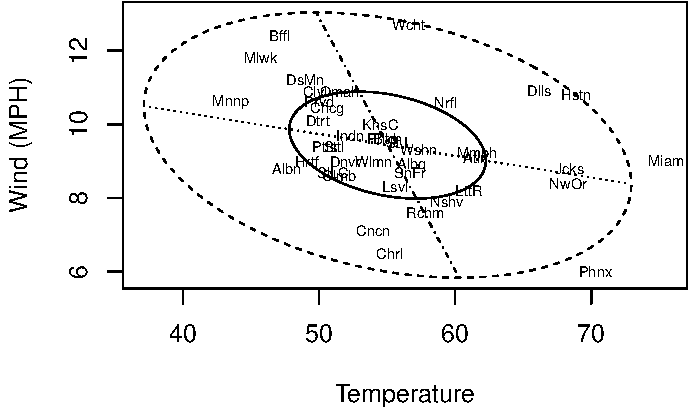
\includegraphics{2.0-Multivariate-Visualization-Assignment_files/figure-latex/unnamed-chunk-4-1} \end{center}

\hypertarget{phoenix-and-miami-are-identified-as-outliers-we-will-perform-a-match-to-obtain-their-positions-and-store-them-in-outcity}{%
\paragraph{\texorpdfstring{\textbf{3. Phoenix and Miami are identified
as outliers, we will perform a match to obtain their positions and store
them in
\texttt{outcity}}}{3. Phoenix and Miami are identified as outliers, we will perform a match to obtain their positions and store them in outcity}}\label{phoenix-and-miami-are-identified-as-outliers-we-will-perform-a-match-to-obtain-their-positions-and-store-them-in-outcity}}

\begin{Shaded}
\begin{Highlighting}[]
\NormalTok{outcity <-}\StringTok{ }\KeywordTok{match}\NormalTok{(}\KeywordTok{c}\NormalTok{(}\StringTok{"Miami"}\NormalTok{, }\StringTok{"Phoenix"}\NormalTok{),}
                 \KeywordTok{rownames}\NormalTok{(USairpollution))}
\end{Highlighting}
\end{Shaded}

\hypertarget{calculate-correlations-with-and-without-these-outliers.}{%
\paragraph{\texorpdfstring{\textbf{4. Calculate correlations with and
without these
outliers.}}{4. Calculate correlations with and without these outliers.}}\label{calculate-correlations-with-and-without-these-outliers.}}

\begin{itemize}
\tightlist
\item
  The correlation drops significantly from -0.35 to -0.26 with the
  outliers removed. This makes sense if you examine the visualization
  and notice that these outliers are generally in line with the
  regression line. Removing them reduces the fit of this line.
\end{itemize}

\begin{Shaded}
\begin{Highlighting}[]
\KeywordTok{cor}\NormalTok{(temp_wind}\OperatorTok{$}\NormalTok{temp, temp_wind}\OperatorTok{$}\NormalTok{wind)}
\end{Highlighting}
\end{Shaded}

\begin{verbatim}
## [1] -0.3497396
\end{verbatim}

\begin{Shaded}
\begin{Highlighting}[]
\KeywordTok{cor}\NormalTok{(temp_wind}\OperatorTok{$}\NormalTok{temp[}\OperatorTok{-}\NormalTok{outcity], temp_wind}\OperatorTok{$}\NormalTok{wind[}\OperatorTok{-}\NormalTok{outcity])}
\end{Highlighting}
\end{Shaded}

\begin{verbatim}
## [1] -0.2587808
\end{verbatim}

\hypertarget{create-the-bivariate-boxplot-for-tempprecip-pair}{%
\paragraph{\texorpdfstring{\textbf{5. Create the bivariate boxplot for
temp/precip
pair}}{5. Create the bivariate boxplot for temp/precip pair}}\label{create-the-bivariate-boxplot-for-tempprecip-pair}}

\begin{Shaded}
\begin{Highlighting}[]
\KeywordTok{bvbox}\NormalTok{(temp_precip, }\DataTypeTok{xlab =} \StringTok{"Temperature"}\NormalTok{, }\DataTypeTok{ylab =} \StringTok{"Precipitation"}\NormalTok{, }\DataTypeTok{type =} \StringTok{"n"}\NormalTok{)}

\KeywordTok{text}\NormalTok{(USairpollution}\OperatorTok{$}\NormalTok{temp, USairpollution}\OperatorTok{$}\NormalTok{precip, }\DataTypeTok{cex =} \FloatTok{0.6}\NormalTok{,}
     \DataTypeTok{labels =} \KeywordTok{abbreviate}\NormalTok{(}\KeywordTok{row.names}\NormalTok{(USairpollution)))}
\end{Highlighting}
\end{Shaded}

\begin{center}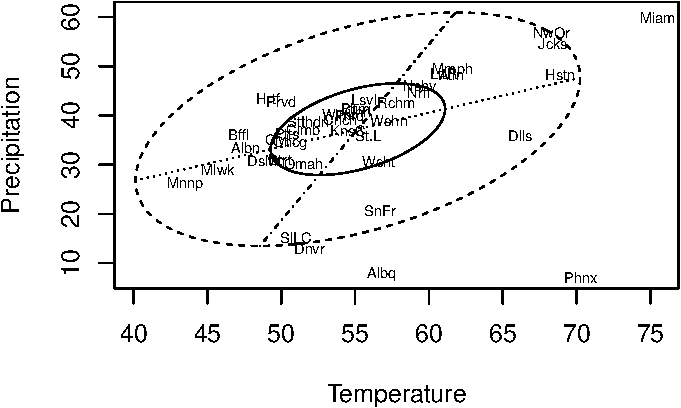
\includegraphics{2.0-Multivariate-Visualization-Assignment_files/figure-latex/unnamed-chunk-7-1} \end{center}

\hypertarget{this-time-we-identify-albuquerque-as-well-as-miami-and-phoenix-as-outliers.-perform-the-same-operation-as-above-to-store-this-in-an-object}{%
\paragraph{\texorpdfstring{\textbf{6. This time we identify Albuquerque
as well as Miami and Phoenix as outliers. Perform the same operation as
above to store this in an
object}}{6. This time we identify Albuquerque as well as Miami and Phoenix as outliers. Perform the same operation as above to store this in an object}}\label{this-time-we-identify-albuquerque-as-well-as-miami-and-phoenix-as-outliers.-perform-the-same-operation-as-above-to-store-this-in-an-object}}

\begin{Shaded}
\begin{Highlighting}[]
\NormalTok{outcity2 <-}\StringTok{ }\KeywordTok{match}\NormalTok{(}\KeywordTok{c}\NormalTok{(}\StringTok{"Miami"}\NormalTok{, }\StringTok{"Phoenix"}\NormalTok{, }\StringTok{"Albuquerque"}\NormalTok{),}
                 \KeywordTok{rownames}\NormalTok{(USairpollution))}
\end{Highlighting}
\end{Shaded}

\hypertarget{calculate-correlations-with-and-without-these-outliers.-1}{%
\paragraph{\texorpdfstring{\textbf{7. Calculate correlations with and
without these
outliers.}}{7. Calculate correlations with and without these outliers.}}\label{calculate-correlations-with-and-without-these-outliers.-1}}

\begin{itemize}
\tightlist
\item
  This time we have the opposite effect; the correlation increases from
  0.39 to 0.62. Looking at the bivariate boxplot, we can see that at
  least two of the outliers are extremely `far' from the regression
  lines.
\end{itemize}

\begin{Shaded}
\begin{Highlighting}[]
\KeywordTok{cor}\NormalTok{(temp_precip}\OperatorTok{$}\NormalTok{temp, temp_precip}\OperatorTok{$}\NormalTok{precip)}
\end{Highlighting}
\end{Shaded}

\begin{verbatim}
## [1] 0.3862534
\end{verbatim}

\begin{Shaded}
\begin{Highlighting}[]
\KeywordTok{cor}\NormalTok{(temp_precip}\OperatorTok{$}\NormalTok{temp[}\OperatorTok{-}\NormalTok{outcity2], temp_precip}\OperatorTok{$}\NormalTok{precip[}\OperatorTok{-}\NormalTok{outcity2])}
\end{Highlighting}
\end{Shaded}

\begin{verbatim}
## [1] 0.6227856
\end{verbatim}

\hypertarget{problem-2}{%
\subsection{Problem 2}\label{problem-2}}

\begin{quote}
The banknote dataset contains measurements on 200 Swiss banknotes: 100
genuine and 100 counterfeits. The variables are the status of the
``note,'' length of the bill, width of the left edge, width of the right
edge, bottom margin width, and top margin width. All measurements are in
millimeters. Read the data and pick the variables: ``note,''
``top\_margin,'' and ``diag\_length.''
\end{quote}

\begin{Shaded}
\begin{Highlighting}[]
\NormalTok{banknote <-}\StringTok{ }\KeywordTok{read.csv}\NormalTok{(}\StringTok{"http://westfall.ba.ttu.edu/isqs6348/Rdata/swiss.csv"}\NormalTok{) }
\NormalTok{notedata <-}\StringTok{ }\NormalTok{banknote[,}\KeywordTok{c}\NormalTok{(}\DecValTok{1}\NormalTok{,}\DecValTok{6}\NormalTok{,}\DecValTok{7}\NormalTok{)]}
\KeywordTok{head}\NormalTok{(notedata)}
\end{Highlighting}
\end{Shaded}

\begin{verbatim}
##   note top_margin diag_length
## 1 real        9.7       141.0
## 2 real        9.5       141.7
## 3 real        9.6       142.2
## 4 real       10.4       142.0
## 5 real        7.7       141.8
## 6 real       10.1       141.4
\end{verbatim}

\hypertarget{a}{%
\subsubsection{A}\label{a}}

\begin{quote}
\begin{enumerate}
\def\labelenumi{\alph{enumi})}
\tightlist
\item
  Construct separate univariate kernel estimates (Gaussian kernel) of
  the distributions of these two variables.
\end{enumerate}
\end{quote}

\hypertarget{first-we-find-the-kernel-density-estimator-of-top_margin-with-the-gaussian-kernel}{%
\paragraph{\texorpdfstring{\textbf{1. First, we find the kernel density
estimator of top\_margin with the Gaussian
kernel:}}{1. First, we find the kernel density estimator of top\_margin with the Gaussian kernel:}}\label{first-we-find-the-kernel-density-estimator-of-top_margin-with-the-gaussian-kernel}}

\begin{Shaded}
\begin{Highlighting}[]
\KeywordTok{plot}\NormalTok{(}\KeywordTok{density}\NormalTok{(notedata}\OperatorTok{$}\NormalTok{top_margin, }\DataTypeTok{bw =} \FloatTok{0.5}\NormalTok{, }\DataTypeTok{kernel =} \StringTok{"gaussian"}\NormalTok{))}
\end{Highlighting}
\end{Shaded}

\begin{center}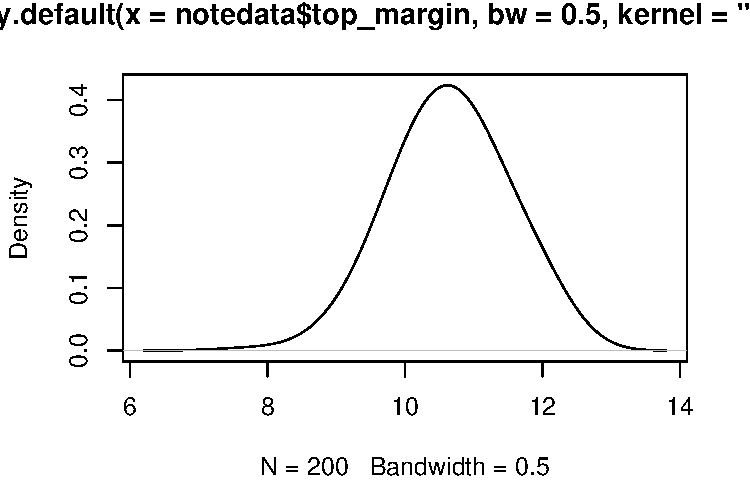
\includegraphics{2.0-Multivariate-Visualization-Assignment_files/figure-latex/unnamed-chunk-11-1} \end{center}

\hypertarget{next-the-same-gaussian-kernel-density-estimator-for-the-diagonal-length}{%
\paragraph{\texorpdfstring{\textbf{2. Next, the same Gaussian kernel
density estimator for the diagonal
length:}}{2. Next, the same Gaussian kernel density estimator for the diagonal length:}}\label{next-the-same-gaussian-kernel-density-estimator-for-the-diagonal-length}}

\begin{Shaded}
\begin{Highlighting}[]
\KeywordTok{plot}\NormalTok{(}\KeywordTok{density}\NormalTok{(notedata}\OperatorTok{$}\NormalTok{diag_length, }\DataTypeTok{bw =} \FloatTok{0.5}\NormalTok{, }\DataTypeTok{kernel =} \StringTok{"gaussian"}\NormalTok{))}
\end{Highlighting}
\end{Shaded}

\begin{center}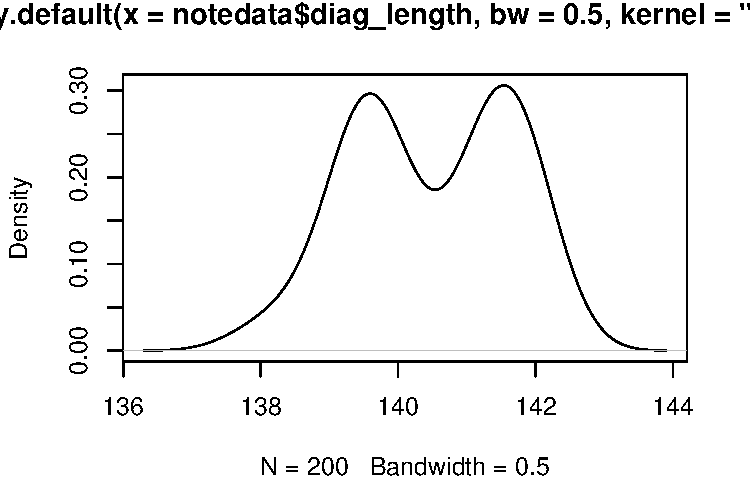
\includegraphics{2.0-Multivariate-Visualization-Assignment_files/figure-latex/unnamed-chunk-12-1} \end{center}

\hypertarget{b}{%
\subsubsection{B}\label{b}}

\begin{quote}
\begin{enumerate}
\def\labelenumi{\alph{enumi})}
\setcounter{enumi}{1}
\tightlist
\item
  Using the bivariate Gaussian kernel, estimate the two variables'
  bivariate density using (i) a contour plot and (ii) a 3-D perspective
  plot.
\end{enumerate}
\end{quote}

\hypertarget{determine-appropriate-bandwidth-for-both-variables-with-dpik}{%
\paragraph{\texorpdfstring{\textbf{1. Determine appropriate bandwidth
for both variables with
\texttt{dpik()}}}{1. Determine appropriate bandwidth for both variables with dpik()}}\label{determine-appropriate-bandwidth-for-both-variables-with-dpik}}

\begin{Shaded}
\begin{Highlighting}[]
\NormalTok{bw <-}\StringTok{ }\KeywordTok{c}\NormalTok{(}\KeywordTok{dpik}\NormalTok{(notedata}\OperatorTok{$}\NormalTok{top_margin), }\KeywordTok{dpik}\NormalTok{(notedata}\OperatorTok{$}\NormalTok{diag_length))}
\end{Highlighting}
\end{Shaded}

\hypertarget{save-the-density-for-contouring}{%
\paragraph{\texorpdfstring{\textbf{2. Save the density for
contouring}}{2. Save the density for contouring}}\label{save-the-density-for-contouring}}

\begin{Shaded}
\begin{Highlighting}[]
\NormalTok{notedimensions <-}\StringTok{ }\NormalTok{notedata[,}\KeywordTok{c}\NormalTok{(}\DecValTok{2}\NormalTok{,}\DecValTok{3}\NormalTok{)]}
\NormalTok{density <-}\StringTok{ }\KeywordTok{bkde2D}\NormalTok{(notedimensions, }\DataTypeTok{bandwidth =}\NormalTok{ bw)}
\end{Highlighting}
\end{Shaded}

\hypertarget{create-the-scatter-plot-with-the-2d-density-contours}{%
\paragraph{\texorpdfstring{\textbf{3. Create the scatter plot with the
(2D) density
contours}}{3. Create the scatter plot with the (2D) density contours}}\label{create-the-scatter-plot-with-the-2d-density-contours}}

\begin{Shaded}
\begin{Highlighting}[]
\KeywordTok{plot}\NormalTok{(notedata}\OperatorTok{$}\NormalTok{top_margin, notedata}\OperatorTok{$}\NormalTok{diag_length,}
     \DataTypeTok{xlab =} \StringTok{"Note Top Margin"}\NormalTok{,}
     \DataTypeTok{ylab =} \StringTok{"Diagonal Note Length"}\NormalTok{,}
     \DataTypeTok{main=}\StringTok{"Swiss Banknote Forgeries"}\NormalTok{)}

\CommentTok{# Add countours}
\KeywordTok{contour}\NormalTok{(}\DataTypeTok{x =}\NormalTok{ density}\OperatorTok{$}\NormalTok{x1, }\DataTypeTok{y =}\NormalTok{ density}\OperatorTok{$}\NormalTok{x2, }\DataTypeTok{z =}\NormalTok{ density}\OperatorTok{$}\NormalTok{fhat, }\DataTypeTok{add =} \OtherTok{TRUE}\NormalTok{)}
\end{Highlighting}
\end{Shaded}

\begin{center}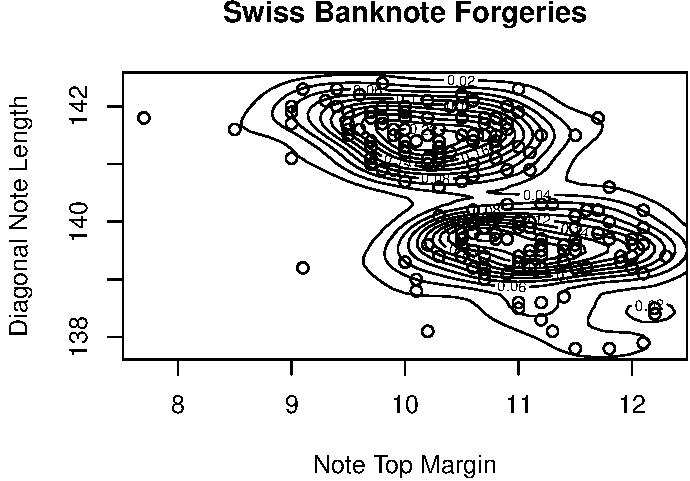
\includegraphics{2.0-Multivariate-Visualization-Assignment_files/figure-latex/unnamed-chunk-15-1} \end{center}

\hypertarget{create-the-scatterplot-with-3d-density-perspective}{%
\paragraph{\texorpdfstring{\textbf{4. Create the scatterplot with 3D
density
perspective}}{4. Create the scatterplot with 3D density perspective}}\label{create-the-scatterplot-with-3d-density-perspective}}

\begin{Shaded}
\begin{Highlighting}[]
\KeywordTok{persp}\NormalTok{(}\DataTypeTok{x =}\NormalTok{ density}\OperatorTok{$}\NormalTok{x1, }\DataTypeTok{y =}\NormalTok{ density}\OperatorTok{$}\NormalTok{x2,}
      \DataTypeTok{z =}\NormalTok{ density}\OperatorTok{$}\NormalTok{fhat,}
      \DataTypeTok{xlab =} \StringTok{"Note Top Margin"}\NormalTok{,}
      \DataTypeTok{ylab =} \StringTok{"Diagonal Note Length"}\NormalTok{,}
      \DataTypeTok{zlab =} \StringTok{"Density"}\NormalTok{,}
      \DataTypeTok{main=}\StringTok{"Swiss Banknote Forgeries"}\NormalTok{, }\DataTypeTok{phi =} \DecValTok{30}\NormalTok{)}
\end{Highlighting}
\end{Shaded}

\begin{center}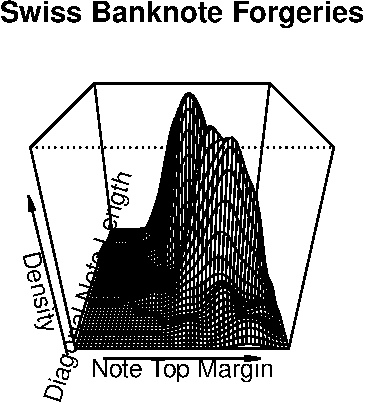
\includegraphics{2.0-Multivariate-Visualization-Assignment_files/figure-latex/unnamed-chunk-16-1} \end{center}

\hypertarget{c}{%
\subsubsection{C}\label{c}}

\begin{quote}
\begin{enumerate}
\def\labelenumi{\alph{enumi})}
\setcounter{enumi}{2}
\tightlist
\item
  Plot the scatterplot, highlighting points with different colors
  according to whether the bills are real or fake (the ``note'' variable
  in the data set has that information). Explain your findings.
\end{enumerate}
\end{quote}

\textbf{We create a simple scatterplot with color codings for real notes
= black and fake notes = red.} - By doing this we can see that this
dataset is not only extremely bimodal, but that these correspond to real
and fake banknotes - The fake banknotes appear to have larger top
margins, but less diagonal length than the real banknotes

\begin{Shaded}
\begin{Highlighting}[]
\CommentTok{# Create plot with color coding}
\KeywordTok{plot}\NormalTok{(notedata[,}\DecValTok{2}\OperatorTok{:}\DecValTok{3}\NormalTok{], }\DataTypeTok{col =} \KeywordTok{ifelse}\NormalTok{(notedata[,}\DecValTok{1}\NormalTok{] }\OperatorTok{==}\StringTok{ "real"}\NormalTok{, }\StringTok{"black"}\NormalTok{, }\StringTok{"red"}\NormalTok{))}

\CommentTok{# Create legend}
\KeywordTok{legend}\NormalTok{(}\StringTok{"topright"}\NormalTok{,}
      \DataTypeTok{legend =} \KeywordTok{c}\NormalTok{(}\StringTok{"real"}\NormalTok{, }\StringTok{"fake"}\NormalTok{),}
      \DataTypeTok{col =} \KeywordTok{c}\NormalTok{(}\StringTok{"black"}\NormalTok{, }\StringTok{"red"}\NormalTok{),}
      \DataTypeTok{pch =} \DecValTok{1}\NormalTok{,}
      \DataTypeTok{cex =} \FloatTok{.8}\NormalTok{)}

\CommentTok{# Add countours}
\KeywordTok{contour}\NormalTok{(}\DataTypeTok{x =}\NormalTok{ density}\OperatorTok{$}\NormalTok{x1, }\DataTypeTok{y =}\NormalTok{ density}\OperatorTok{$}\NormalTok{x2, }\DataTypeTok{z =}\NormalTok{ density}\OperatorTok{$}\NormalTok{fhat, }\DataTypeTok{add =} \OtherTok{TRUE}\NormalTok{)}
\end{Highlighting}
\end{Shaded}

\begin{center}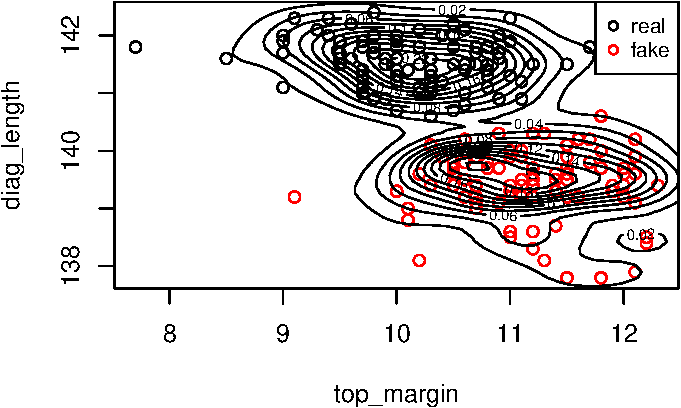
\includegraphics{2.0-Multivariate-Visualization-Assignment_files/figure-latex/unnamed-chunk-17-1} \end{center}

\hypertarget{problem-3}{%
\subsection{Problem 3}\label{problem-3}}

\begin{quote}
Examine the multivariate normality (MVN) of the banknote data (excluding
the ``note'' variable) by creating the chi-square plot of the data. Load
the data as follow. Follow the listed steps to examine the multivariate
normality.
\end{quote}

\begin{Shaded}
\begin{Highlighting}[]
\NormalTok{notedata2 <-}\StringTok{ }\NormalTok{banknote[,}\OperatorTok{-}\DecValTok{1}\NormalTok{]}
\KeywordTok{head}\NormalTok{(notedata2)}
\end{Highlighting}
\end{Shaded}

\begin{verbatim}
##   length left_width right_width bottom_margin top_margin diag_length
## 1  214.8      131.0       131.1           9.0        9.7       141.0
## 2  214.6      129.7       129.7           8.1        9.5       141.7
## 3  214.8      129.7       129.7           8.7        9.6       142.2
## 4  214.8      129.7       129.6           7.5       10.4       142.0
## 5  215.0      129.6       129.7          10.4        7.7       141.8
## 6  215.7      130.8       130.5           9.0       10.1       141.4
\end{verbatim}

\hypertarget{a-find-the-column-means-vector.}{%
\subsubsection{A) Find the column-means
vector.}\label{a-find-the-column-means-vector.}}

\textbf{Here we find the column means and store them in Xbar}

\begin{Shaded}
\begin{Highlighting}[]
\NormalTok{xbar <-}\StringTok{ }\KeywordTok{colMeans}\NormalTok{(notedata2)}
\NormalTok{xbar}
\end{Highlighting}
\end{Shaded}

\begin{verbatim}
##        length    left_width   right_width bottom_margin    top_margin 
##      214.8960      130.1215      129.9565        9.4175       10.6505 
##   diag_length 
##      140.4835
\end{verbatim}

\hypertarget{b-find-the-covariance-matrix-of-the-data.}{%
\subsubsection{B) Find the covariance matrix of the
data.}\label{b-find-the-covariance-matrix-of-the-data.}}

** Save the covariance of our Swiss notes data in S:**

\begin{Shaded}
\begin{Highlighting}[]
\NormalTok{S <-}\StringTok{ }\KeywordTok{cov}\NormalTok{(notedata2)}
\NormalTok{S}
\end{Highlighting}
\end{Shaded}

\begin{verbatim}
##                    length  left_width right_width bottom_margin top_margin
## length         0.14179296  0.03144322  0.02309146    -0.1032462 -0.0185407
## left_width     0.03144322  0.13033945  0.10842739     0.2158028  0.1050394
## right_width    0.02309146  0.10842739  0.16327412     0.2841319  0.1299967
## bottom_margin -0.10324623  0.21580276  0.28413191     2.0868781  0.1645389
## top_margin    -0.01854070  0.10503945  0.12999673     0.1645389  0.6447234
## diag_length    0.08430553 -0.20934196 -0.24047010    -1.0369962 -0.5496148
##               diag_length
## length         0.08430553
## left_width    -0.20934196
## right_width   -0.24047010
## bottom_margin -1.03699623
## top_margin    -0.54961482
## diag_length    1.32771633
\end{verbatim}

\hypertarget{c-find-the-mahalanobis-distances-given-using-the-data-and-the-result-of-parts-a-and-b.}{%
\subsubsection{C) Find the Mahalanobis distances given using the data
and the result of parts a and
b.}\label{c-find-the-mahalanobis-distances-given-using-the-data-and-the-result-of-parts-a-and-b.}}

\textbf{Using the \texttt{mahalanobis()} function, we plug in the data
with the column means and covariance to find the Mahalanobis distances:}

\begin{Shaded}
\begin{Highlighting}[]
\NormalTok{d2 <-}\StringTok{ }\KeywordTok{mahalanobis}\NormalTok{(notedata2, xbar, S)}
\NormalTok{d2}
\end{Highlighting}
\end{Shaded}

\begin{verbatim}
##   [1] 24.1822330  4.4554815  3.3862349  2.8429463 17.4722855  9.3219107
##   [7]  9.8042238  5.7728142  8.5299136  3.1996948  9.6407351  5.4062400
##  [13] 17.4950978  3.7504885  2.6343394 10.3456632  6.2974792  4.2870447
##  [19]  7.7004403  4.0536247  3.6330789  5.9255552  6.4372035  5.1073406
##  [25]  5.1089894  9.6852215  6.1461050  6.0985269  3.3328174  5.2250235
##  [31]  2.6551357  4.9356472  2.7281070  4.3450616  8.1854385  6.3338524
##  [37]  4.5880792  3.9323394  6.0046395 28.4939129  8.3845177  2.5361408
##  [43]  5.3738641  5.3809814  6.0594238  5.2350319  1.0980743  4.2016621
##  [49]  3.7321367 14.9317002  4.9166117  6.1811642  4.3628039  4.7271556
##  [55]  5.4578142  4.9743699 10.1261952  7.4588354  1.9647956  0.9801036
##  [61]  3.7165107  4.3121951  5.0359862  4.7084987  1.1686711  4.2677333
##  [67]  4.3789534  3.7423529  4.4801803  5.2534522 11.4668468  2.3030182
##  [73]  9.9720370  5.4007099  3.3740429  8.5119132  3.1278829  3.9106167
##  [79]  5.6256017  3.9169904  3.4100169  2.7745593  7.6604553  1.7542228
##  [85]  6.9110882  1.6180346  2.7126363  5.1216222  5.3262090  2.2888119
##  [91]  3.3487717  3.5331891  4.8545708  4.9628844  2.8134114  6.3416884
##  [97]  2.8217861  3.5043815  1.1821895  4.4416822  4.8431122  2.9901218
## [103]  2.4448228  3.3937963  3.6264349  1.1502206  5.9386644  3.6549450
## [109]  4.1826648  5.9051392  7.2361317  3.5312284 13.6721778  5.2237190
## [115]  1.8236887  8.9013403  5.9074713  4.9394296  2.7285680  5.1370863
## [121]  4.3177627  6.1828397 11.2545134  2.8181005  4.6186889  3.8217062
## [127]  2.6596084  7.3967043  2.1095077  8.9522262  3.3024746  8.0516287
## [133]  3.0533084  4.4710959  5.3391935  4.5188320  5.8781588  9.2269819
## [139]  2.9444483  5.3028022  3.1001636  7.0968556  3.3780129  1.6926028
## [145]  6.7357690  4.2728377  2.7194444 10.9317315  1.1955684  7.4720971
## [151]  5.2551247  8.0500047  8.4150356  4.8141217  3.8406819  6.3366302
## [157]  6.5304754  3.3376580  7.7133550 15.9965806 21.4697051 14.5249697
## [163]  2.7899519  3.4533610  4.7555441  6.1859662 25.1679604 10.1836802
## [169]  5.1673717  3.9762942 25.6509644  9.4815329  3.3033659  9.8294635
## [175]  2.6094774  3.6080347  4.3702953  5.5375330  3.5997698 18.7619304
## [181]  3.2896745 13.7484228  3.3646008  2.7510298  1.1711986  3.4171748
## [187] 11.6212331  5.3446211  5.7222961 12.6440935  6.7329757 13.0130250
## [193]  1.4372402  6.5388802  3.8545002  3.7402127  3.6216497  1.9835372
## [199]  5.4698103  4.1498014
\end{verbatim}

\hypertarget{d-sort-the-mahalanobis-distances-from-smallest-to-largest.}{%
\subsubsection{D) Sort the Mahalanobis distances from smallest to
largest.}\label{d-sort-the-mahalanobis-distances-from-smallest-to-largest.}}

\textbf{Sort the distances to see which are the closest and furthest
from the mean. Save into sorted\_d2 for future use.}

\begin{Shaded}
\begin{Highlighting}[]
\NormalTok{sorted_d2 <-}\StringTok{ }\KeywordTok{sort}\NormalTok{(d2, }\DataTypeTok{decreasing =} \OtherTok{FALSE}\NormalTok{) }
\end{Highlighting}
\end{Shaded}

\hypertarget{e-chi-square-distribution}{%
\subsubsection{E) Chi-Square
Distribution}\label{e-chi-square-distribution}}

\begin{quote}
Suppose your data is multivariate normal, by definition. In that case,
the Mahalanobis distances should follow the chi-sq distribution (with df
= number of columns), so create a chi-square quantile values list and
plot them vs.~the sorted Mahalanobis distances. The quantiles should be
on the x-axis, and the sorted Mahalonobis distances must be on the
y-axis. Please label your chart correctly. You also need to add a
45-degree line to your plot by running this code abline(a = 0, b = 1)
after the plot code.
\end{quote}

** Create a chi-square distribution to plot against the sorted
Mahalanobis distances. We add a 45-degree line to see how close our
squared distances are to the line.**

\begin{Shaded}
\begin{Highlighting}[]
\CommentTok{# For concise code, store notedata2 in x }
\NormalTok{x <-}\StringTok{ }\NormalTok{notedata2}

\CommentTok{# Define the chi square distribution}
\NormalTok{quantiles <-}\StringTok{ }\KeywordTok{qchisq}\NormalTok{((}\DecValTok{1}\OperatorTok{:}\KeywordTok{nrow}\NormalTok{(x) }\OperatorTok{-}\StringTok{ }\DecValTok{1}\OperatorTok{/}\DecValTok{2}\NormalTok{) }\OperatorTok{/}\StringTok{ }\KeywordTok{nrow}\NormalTok{(x), }\DataTypeTok{df =} \KeywordTok{ncol}\NormalTok{(x))}

\CommentTok{# Plot chi square against sorted distances}
\KeywordTok{plot}\NormalTok{(quantiles, sorted_d2,}
\DataTypeTok{xlab =} \KeywordTok{expression}\NormalTok{(}\KeywordTok{paste}\NormalTok{(chi[}\DecValTok{3}\NormalTok{]}\OperatorTok{^}\DecValTok{2}\NormalTok{, }\StringTok{" Quantile"}\NormalTok{)), }\DataTypeTok{ylab =} \StringTok{"Ordered squared distances"}\NormalTok{)}

\CommentTok{# Add 45 degree reference line }
\KeywordTok{abline}\NormalTok{(}\DataTypeTok{a =} \DecValTok{0}\NormalTok{, }\DataTypeTok{b =} \DecValTok{1}\NormalTok{)}
\end{Highlighting}
\end{Shaded}

\begin{center}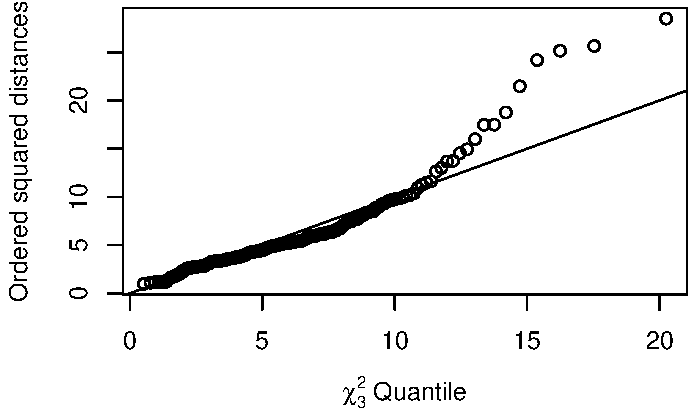
\includegraphics{2.0-Multivariate-Visualization-Assignment_files/figure-latex/unnamed-chunk-23-1} \end{center}

\hypertarget{f-interpret-the-plot-of-part-e.-is-the-data-mvn}{%
\subsubsection{F) Interpret the plot of part e. Is the data
MVN?}\label{f-interpret-the-plot-of-part-e.-is-the-data-mvn}}

\textbf{Based on the closeness of the data to the reference line and
zero, the data does appear to be a multivariate normal distribution.}

\hypertarget{problem-4}{%
\subsection{Problem 4}\label{problem-4}}

\begin{quote}
Use TTU graduate student exit survey data to answer the following
questions.
\end{quote}

\begin{Shaded}
\begin{Highlighting}[]
\NormalTok{grad <-}\StringTok{ }\KeywordTok{read.csv}\NormalTok{(}\StringTok{"http://westfall.ba.ttu.edu/isqs6348/Rdata/pgs.csv"}\NormalTok{)}
\end{Highlighting}
\end{Shaded}

\hypertarget{a-this-data-contains-a-rating-of-how-many-students}{%
\subsubsection{A) This data contains a rating of how many
students?}\label{a-this-data-contains-a-rating-of-how-many-students}}

\textbf{This dataset contains ratings from 2002 students:}

\begin{Shaded}
\begin{Highlighting}[]
\KeywordTok{nrow}\NormalTok{(grad)}
\end{Highlighting}
\end{Shaded}

\begin{verbatim}
## [1] 2002
\end{verbatim}

\hypertarget{b-make-a-scatterplot-of-facteaching-and-facknowledge}{%
\subsubsection{B) Make a scatterplot of ``Facteaching'' and
``FacKnowledge''}\label{b-make-a-scatterplot-of-facteaching-and-facknowledge}}

\begin{quote}
If your plot looks odd, use jitter() of each variable, then plot.
\end{quote}

\textbf{Plotting the scores of faculty teaching and knowledge against
each other results in an unhelpful plot, so we add a \texttt{jitter()}
so add some noise and see individual datapoints more easily:}

\begin{Shaded}
\begin{Highlighting}[]
\KeywordTok{plot}\NormalTok{(}\KeywordTok{jitter}\NormalTok{(grad}\OperatorTok{$}\NormalTok{FacTeaching), }\KeywordTok{jitter}\NormalTok{(grad}\OperatorTok{$}\NormalTok{FacKnowledge),}
     \DataTypeTok{xlab =} \StringTok{"Faculty Teaching Rating"}\NormalTok{,}
     \DataTypeTok{ylab =} \StringTok{"Faculty Knowledge Rating"}\NormalTok{,}
     \DataTypeTok{main =} \StringTok{"Faculty Teaching vs Knowledge"}\NormalTok{)}
\end{Highlighting}
\end{Shaded}

\begin{center}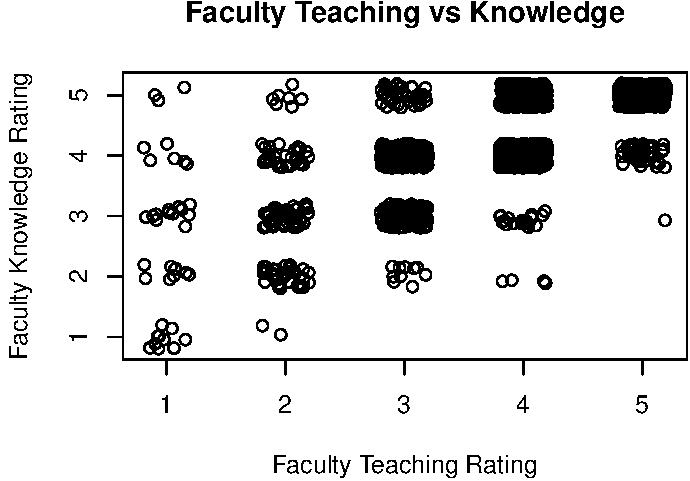
\includegraphics{2.0-Multivariate-Visualization-Assignment_files/figure-latex/unnamed-chunk-26-1} \end{center}

\hypertarget{c-create-new-dataframe-for-facteaching-facknowledge-and-housing}{%
\subsubsection{C) Create new dataframe for ``FacTeaching,''
``FacKnowledge'', and
``Housing''}\label{c-create-new-dataframe-for-facteaching-facknowledge-and-housing}}

\textbf{Let's create an object with these three variables so we can
compare them in the next section:}

\begin{Shaded}
\begin{Highlighting}[]
\NormalTok{grad_3var <-}\StringTok{ }\NormalTok{grad[,}\KeywordTok{c}\NormalTok{(}\StringTok{"FacTeaching"}\NormalTok{, }\StringTok{"FacKnowledge"}\NormalTok{, }\StringTok{"Housing"}\NormalTok{)]}
\end{Highlighting}
\end{Shaded}

\hypertarget{d-find-a-correlation-matrix-for-the-data-of-part-c.}{%
\subsubsection{D) Find a correlation matrix for the data of part
(c).}\label{d-find-a-correlation-matrix-for-the-data-of-part-c.}}

\begin{quote}
If there are NAs (missing values) in your data, estimate the correlation
matrix by all three following methods.
\end{quote}

\textbf{Let's attempt a correlation first to see if it will calculate:}
- Spoiler: it did not. It's time to handle some nulls!

\begin{Shaded}
\begin{Highlighting}[]
\KeywordTok{cor}\NormalTok{(grad_3var)}
\end{Highlighting}
\end{Shaded}

\begin{verbatim}
##              FacTeaching FacKnowledge Housing
## FacTeaching            1           NA      NA
## FacKnowledge          NA            1      NA
## Housing               NA           NA       1
\end{verbatim}

\hypertarget{i.-complete-case-analysis.}{%
\paragraph{i. Complete-case
analysis.}\label{i.-complete-case-analysis.}}

\textbf{First we will calculate the correlation using complete-case
analysis, which deletes all rows that contain any NAs.}

\begin{Shaded}
\begin{Highlighting}[]
\KeywordTok{cor}\NormalTok{(}\KeywordTok{na.omit}\NormalTok{(grad_3var))}
\end{Highlighting}
\end{Shaded}

\begin{verbatim}
##              FacTeaching FacKnowledge   Housing
## FacTeaching    1.0000000    0.7113826 0.1536942
## FacKnowledge   0.7113826    1.0000000 0.2108483
## Housing        0.1536942    0.2108483 1.0000000
\end{verbatim}

\hypertarget{ii.-available-case-analysis.}{%
\paragraph{ii. Available-case
analysis.}\label{ii.-available-case-analysis.}}

\textbf{Next we calculate the correlation matrix using available-case,
or ``pairwise'' analysis:}

\begin{Shaded}
\begin{Highlighting}[]
\KeywordTok{cor}\NormalTok{(grad_3var, }\DataTypeTok{use =} \StringTok{"pairwise"}\NormalTok{)}
\end{Highlighting}
\end{Shaded}

\begin{verbatim}
##              FacTeaching FacKnowledge   Housing
## FacTeaching    1.0000000    0.7109232 0.1556915
## FacKnowledge   0.7109232    1.0000000 0.2102034
## Housing        0.1556915    0.2102034 1.0000000
\end{verbatim}

\hypertarget{iii.-maximum-likelihood-estimation.}{%
\paragraph{iii. Maximum likelihood
estimation.}\label{iii.-maximum-likelihood-estimation.}}

\textbf{Using the \texttt{norm} package, we can calculate the maximum
likelihood estimate:}

\begin{Shaded}
\begin{Highlighting}[]
\NormalTok{pre <-}\StringTok{ }\KeywordTok{prelim.norm}\NormalTok{(}\KeywordTok{as.matrix}\NormalTok{(grad_3var))}
\NormalTok{theta_hat <-}\StringTok{ }\KeywordTok{em.norm}\NormalTok{(pre)}
\end{Highlighting}
\end{Shaded}

\begin{verbatim}
## Iterations of EM: 
## 1...2...3...4...5...6...
\end{verbatim}

\begin{Shaded}
\begin{Highlighting}[]
\NormalTok{ml.fit <-}\StringTok{ }\KeywordTok{getparam.norm}\NormalTok{(pre,theta_hat)}
\end{Highlighting}
\end{Shaded}

\begin{Shaded}
\begin{Highlighting}[]
\NormalTok{corr.ml <-}\StringTok{ }\KeywordTok{cov2cor}\NormalTok{(ml.fit}\OperatorTok{$}\NormalTok{sigma)}
\NormalTok{corr.ml}
\end{Highlighting}
\end{Shaded}

\begin{verbatim}
##           [,1]      [,2]      [,3]
## [1,] 1.0000000 0.7120454 0.1541005
## [2,] 0.7120454 1.0000000 0.2103328
## [3,] 0.1541005 0.2103328 1.0000000
\end{verbatim}

\hypertarget{is-there-a-noticeable-difference-between-the-three-methods-of-missing-value-treatment-which-method-do-you-suggest}{%
\paragraph{Is there a noticeable difference between the three methods of
missing value treatment? Which method do you
suggest?}\label{is-there-a-noticeable-difference-between-the-three-methods-of-missing-value-treatment-which-method-do-you-suggest}}

The correlation matrices are extremely close, in this case it appears
that any of these methods would give you an accurate value. From this, I
would speculate that there are few nulls in the data.

This could be because some responses are enforced through the survey
software, or that students don't feel the need to skip questions.
However, knowing that our data is distributed fairly normally it would
be best to use maximum likelihood estimates to impute these nulls.

\end{document}
